
\Universita{UNIVERSITY OF TRENTO}
\CorsoDiLaurea{Master's Degree in Data Science}
\AnnoAccademico{2025-2026}
\Titolo{Secure LLM orchestration for \ enterprise workflows using the \ Model Context Protocol}
\Relatore{Prof. Daniele Miorandi}
\RelatoreLabel{Supervisor}
\CandidatoLabel{Graduate Student}

\Candidato{Ettore Miglioranza} 
\Matricola{257311}
\DataEsame{\today}
\Logo{Impaginazione/logo_rosso.png}
\LogoWidth{4.5cm} %optional, default: 3cm
\LogoPosition{top}
\LogoSfondo{Impaginazione/logo_bn.png}
\opacitaSfondo{0.05}

\begin{titlepage}
    \newgeometry{left=3cm, right=3cm, bottom=2cm, top =3cm} 
    \pagestyle{empty}
    \makefrontpage
    \restoregeometry
\end{titlepage}


\newpage
\thispagestyle{empty}
\mbox{}  % This ensures an empty page
\newpage


\frontmatter
% dedica
\null\vspace{\stretch{1}}
\begin{flushright}
    \textit{Dedica}
\end{flushright}
\vspace{\stretch{2}}\null

%ringraziamenti
\chapter*{Acknowledgments}

%I would like to thank my supervisor, Prof. Daniele Miorandi, for his guidance and continuous support throughout this thesis work.


\begin{abstract}
Large language models (LLMs) have demonstrated cutting-edge capabilities in understanding intent and semantic routing, but their adoption in business workflows remains limited by stringent privacy and security requirements. This thesis investigates how LLM-based orchestration can be implemented in a real-world business context, whilst providing a formal guarantee that no personally identifiable information (PII) crosses the boundaries of an external model. The work focuses on a specific workforce management domain within the Antares ERP ecosystem, where natural language requests must be reliably mapped to operational actions, such as locating nearby workers on construction sites, identifying colleagues based on proximity, and validating absence cover and substitution chains. 

The central research question is: how can an external LLM be integrated as a semantic router without exposing sensitive business data, whilst ensuring deterministic and verifiable execution of business tools? To answer this question, the thesis proposes a ‘privacy-by-design’ architecture based on the Model Context Protocol (MCP). The system enforces a strict separation between language understanding and data access through a reversible anonymisation pipeline: user requests are pseudonymised before reaching the model, routed by the LLM using only anonymised text, and de-anonymised exclusively on the server side at the time of tool execution. Entity detection is performed by a multilingual NER microservice based on GLiNER, chosen over rule-based alternatives such as Microsoft Presidio precisely because of its robustness in processing business inputs in Italian. Token-to-entity mappings are stored in a short-lived Redis context, ensuring that pseudonymisation is both ephemeral and fully reversible. The MCP server exposes schema-validated, typed tools to the model and enforces strict routing constraints, whilst a \texttt{.NET 10} client orchestrator manages the end-to-end request lifecycle. 

The approach draws on the broader state of the art in privacy-preserving LLM infrastructure. In particular, OpenAI’s Privacy Filter (Apache 2.0, 2025), recently made open source, confirms that lightweight, on-premise NER models incorporated as pre-processing layers represent the emerging industry standard for PII containment. The key architectural contribution of this thesis relative to that reference model is \emph{reversibility}: whilst one-way encoding destroys the mapping between placeholders and entities, the token-based scheme proposed here preserves full operational correctness whilst allowing controlled de-anonymisation at the protocol boundary, a distinction relevant under Article 4.5 of the GDPR, which classifies such processing as pseudonymisation rather than anonymisation.  

The thesis makes three concrete contributions: (1) a multi-service architecture that structurally isolates sensitive data from the LLM context, (2) a deterministic and reversible privacy layer based on token mapping that preserves the correctness of business logic throughout the entire request lifecycle, and (3) a validated set of realistic workforce management use cases demonstrating the effectiveness of the approach in a representative production environment. The validation confirms that the accuracy of semantic routing and NER performance on Italian-language inputs are sufficient for enterprise deployment and that no raw PII is observable within the boundaries of the tested LLM context. 

This work positions MCP as a practical and applicable interface standard for enterprise AI orchestration and highlights the key engineering trade-off inherent in privacy by design: increased architectural complexity is the necessary cost for demonstrable privacy assurance, but it unlocks reliable and verifiable LLM-driven workflows without violating data protection constraints.

\vspace{1em}
\noindent\textbf{Keywords:} LLM orchestration, Model Context Protocol (MCP), privacy-by-design, PII pseudonymization, semantic routing, named entity recognition, GLiNER, enterprise AI security, GDPR compliance
\end{abstract}

\tableofcontents

\mainmatter

\input{capitoli/introduction}

\chapter{Background and Related Work}
\label{ch:background}

This chapter reviews the three bodies of literature that inform the design of the system presented in subsequent chapters: the integration of large language models into enterprise software, the Model Context Protocol as a standardisation layer for LLM tool interfaces, and privacy-preserving natural language processing with a focus on named entity recognition and PII protection. Section~\ref{sec:background_llm_enterprise} examines how large language models change semantic routing and tool invocation in enterprise systems, and the engineering constraints that shift introduces. Section~\ref{sec:background_mcp} turns to the Model Context Protocol and the security boundaries it defines between client, server, and model. Section~\ref{sec:background_privacy_nlp} addresses the regulatory and technical grounding of PII protection, from the GDPR's definition of personal data to detection approaches ranging from rule-based systems to zero-shot transformers. Section~\ref{sec:background_sota} surveys the current state of the art in secure LLM orchestration and identifies the gap that motivates this work.

% ==========================================
\section{Large Language Models in Enterprise Workflows}
\label{sec:background_llm_enterprise}

The modern generation of large language models traces its architectural lineage to the transformer, introduced by Vaswani et al.~\cite{vaswani2017attention} in 2017. The attention mechanism, which allows each token in a sequence to attend to every other token, proved to be the basis for a qualitative leap in language understanding. Scaling transformer-based models, exemplified by GPT-3~\cite{brown2020language} with its 175 billion parameters, showed that sufficiently large models exhibit capabilities not present in smaller counterparts: multi-step reasoning, few-shot generalisation from in-context examples, and reliable instruction following across diverse domains~\cite{wei2022emergent}. Instruction following is not an emergent side effect of scale alone; it is the product of a dedicated post-training step, reinforcement learning from human feedback, that fine-tunes a base model specifically to follow natural-language instructions rather than merely continue text~\cite{ouyang2022instructgpt}. That step is what makes a natural-language tool description usable as a routing signal at all: a base model without it would have no learned tendency to treat a sentence such as ``call \texttt{get\_colleagues\_of\_person} when the user asks about coworkers'' as an instruction to act on.

For enterprise software, the practical implication is a new paradigm for human-system interaction. Until recently, bridging the gap between a user's natural language expression and a system's formal data operations required rule engines, supervised intent classifiers, or custom NLP pipelines. A general-purpose language model can close that gap from the prompt alone, interpreting natural language requests and mapping them to well-typed business operations without labelled training data or domain-specific engineering.

The shift creates real engineering problems. Enterprise workflows demand deterministic, auditable outputs. Sensitive business data must not be transmitted to third-party model providers. System behaviour must remain predictable under adversarial or malformed inputs. These constraints sit in direct tension with the generative, probabilistic nature of LLMs, and reconciling them is an active area of research and engineering.

\subsection{Semantic Routing and Intent Classification}
\label{subsec:background_semantic_routing}

Semantic routing refers to interpreting a natural language utterance and directing it to the appropriate downstream component based on its inferred intent. Classical approaches used supervised intent classifiers trained on labelled utterance datasets~\cite{larson2019evaluation}. These models required curated training data per domain and were brittle under paraphrasing, multilingual input, or out-of-distribution requests. In practice, that limitation has a direct cost: adding a new business action, or supporting a new language, means collecting and labelling a fresh batch of example utterances before the classifier can be retrained and redeployed, a cost that scales with every intent and every language a deployment needs to cover.

LLMs remove that cost. Because they acquire broad linguistic knowledge during pre-training, they can classify intent zero-shot given only a natural language description of the available actions, with no labelled dataset and no retraining step. Routing logic becomes a prompt rather than a trained artefact, and adding a new action or language is a matter of editing text, not collecting data. A recent example, though outside classic intent classification, is a conversational, RAG-based assistant for AI-supported document creation workflows~\cite{dalia2025workflow}, which replaces a rule-based document generation flow with natural-language interaction end-to-end. The saving is not free, however. The quality of zero-shot routing depends heavily on the specificity and clarity of tool descriptions, and vague or overlapping descriptions cause the model to route incorrectly regardless of the underlying model's capability, making prompt engineering a first-class concern in deployed systems. Recent work on agentic tool selection confirms the sensitivity directly: editing only a tool's description, with its underlying functionality unchanged, can shift how often an LLM selects that tool over a competing one by an order of magnitude~\cite{faghih2025toolpreferences}.

\subsection{Tool Calling and AI Agents}
\label{subsec:background_tool_calling}

The capacity for LLMs to invoke external functions (also called function calling) was formalised as a first-class API feature by major model providers in 2023, part of a broader shift towards treating tool use as a core capability rather than a prompting trick~\cite{qu2024toollearning}. In this paradigm, the developer supplies the model with a schema describing callable functions, their parameters and return types. The model produces a structured call rather than free text; the host application executes it and feeds the result back for the model to incorporate into its response.

The ReAct framework~\cite{yao2023react} formalised the interleaving of reasoning traces and tool invocations, showing that a model that explicitly reasons about which tool to call outperforms models that invoke tools without intermediate reasoning, especially in multi-step tasks. This is the AI agent paradigm: a language model acting as an orchestrator that selects and sequences tool calls to reach a higher-level goal.

The Toolformer work~\cite{schick2023toolformer} showed that models can learn to use external APIs from self-supervised examples, acquiring tool use directly from patterns in text rather than from an explicit interface definition. Nothing in that training signal constrains the resulting call to a fixed, machine-checkable format: a malformed or incomplete invocation is not distinguishable, from the model's own output, from a well-formed one. That gap is not cosmetic in an enterprise setting. A routing decision that cannot be validated against a schema cannot be logged in a structured, replayable form, and there is no reliable way to confirm after the fact which tool was called with which parameters. Later systems such as Gorilla~\cite{patil2023gorilla} narrowed the correctness gap by fine-tuning a model on API documentation and evaluating calls by execution rather than surface similarity, but the underlying call is still free text scored after the fact, not structurally guaranteed beforehand. For this reason, enterprise deployments generally prefer explicit schema-driven invocation over learned tool use. Schema-driven invocation provides stronger output format guarantees and makes the routing decision auditable.

Two architectural properties of tool-calling systems have direct implications for enterprise deployments. First, the model's agency can be bounded by restricting which tools it may call: exposing only business-level operations and keeping data access inside deterministic code limits the model to intent classification and parameter extraction. Second, the tool result feedback loop, in which tool outputs are returned to the model for further reasoning, is the primary vector for indirect prompt injection attacks~\cite{greshake2023not}, making its design a security-relevant decision.

% ==========================================
\section{The Model Context Protocol (MCP)}
\label{sec:background_mcp}

The Model Context Protocol~\cite{anthropic2024mcp}, published by Anthropic in November 2024, standardises the communication interface between LLM client applications and external tool servers. Before MCP, each LLM-tool integration required bespoke glue code, custom serialisation formats, and proprietary conventions. MCP defines a vendor-neutral interface so that any compliant client can connect to any compliant server without integration-specific adaptation.

The design is modelled after the Language Server Protocol (LSP)~\cite{microsoft2024lsp,bunder2019decoupling}, which eliminated the $N \times M$ explosion of editor-language integrations by decoupling language-analysis servers from editor clients. MCP applies the same logic: any client that speaks MCP can talk to any server that speaks MCP, reducing the integration surface from $N \times M$ to $N + M$.

\subsection{Standardising LLM Interfaces}
\label{subsec:background_mcp_standardization}

MCP defines three categories of server-exposed primitives~\cite{anthropic2024mcp}. \emph{Tools} are callable functions with typed input schemas and structured return values, analogous to OpenAPI operations. \emph{Resources} are read-only data sources the model can pull into its context: file contents, database records, configuration objects. \emph{Prompts} are reusable, parameterised message templates.

Communication runs over two transports: standard input/output for locally spawned server processes, and HTTP with Server-Sent Events (SSE) for network-accessible servers. The underlying message format is JSON-RPC~2.0~\cite{jsonrpc2010spec}, a stateless, language-agnostic remote procedure call protocol that predates MCP by over a decade; MCP reuses it as a wire format rather than defining a new one. Tool schemas are JSON Schema objects describing parameter types, constraints, and documentation. This standardised schema representation allows tooling to auto-generate type-safe client code from server definitions, reducing the risk of schema drift between client expectations and server implementation.

\subsection{Security Boundaries in MCP}
\label{subsec:background_mcp_security}

MCP's security model separates three roles. The \emph{MCP host} manages client connections and controls which servers the model may reach. The \emph{MCP server} is a trusted executor with access to real data and infrastructure. The \emph{model} is a semantic reasoner: it produces structured tool calls but accesses no data source directly. This separation exists to avoid a specific, decades-old failure mode: the confused deputy problem, in which a component with legitimate access to a resource is tricked by a less-privileged caller into misusing that access on the caller's behalf~\cite{hardy1988confuseddeputy}. A model that could both reason over untrusted input and act directly on sensitive data would be exactly this kind of deputy; keeping data access confined to the server, and never handing the model direct authority over it, is what keeps that failure mode structurally unavailable rather than merely discouraged.

This three-layer separation creates a natural enforcement point for privacy, but only for data at rest: the server is the only component with direct access to backend data and infrastructure. It says nothing about the raw text of a user's request, which in plain MCP still passes through the host to the model exactly as typed, PII included, since nothing in the protocol itself intercepts it first. A pre-processing step applied to user requests before they reach the model can close that specific gap, structurally preventing PII from entering the LLM context, because the server's trust boundary sits downstream of the model. The model then operates only on what that pre-processing step lets through, not on the raw request itself.

Prompt injection~\cite{greshake2023not} is the primary known attack on this architecture. Malicious content embedded in tool results or externally retrieved resources can attempt to hijack the model's behaviour by simulating system-level instructions. Mitigations include restricting the model's tool set, limiting the scope of requests the model may issue, and routing business logic through deterministic code that does not re-enter the model after execution. These mitigations reduce the attack surface but do not eliminate it, and the design of the tool result feedback loop remains an open security concern in MCP deployments. A systematic security analysis of the MCP ecosystem~\cite{hou2025mcpsecurity} catalogues these risks across the full server lifecycle, from malicious tool registration to compromised transport, and finds that few real deployments implement the safeguards it recommends.

MCP has moved through more than one revision since this project's implementation began. The system described in this thesis targets the original November 2024 specification~\cite{anthropic2024mcp}; the current stable revision at the time of writing is dated 2025-11-25~\cite{mcp2025specnov}. Two differences between the two matter for the architecture in Chapter~\ref{ch:architecture}. Transport: the original spec used HTTP with Server-Sent Events (HTTP+SSE), described above. An intermediate 2025-03-26 revision replaced it with Streamable HTTP, a single-endpoint transport superseding the original's paired POST/GET-and-long-lived-connection design; HTTP+SSE is deprecated for new implementations and kept only for backward compatibility. Authorisation: the current specification adds an OAuth~2.1-based authorisation framework~\cite{ietf2025oauth21}, absent from the November 2024 baseline this project's MCP server implements. Neither difference changes the security argument made in this section, the enforcement point still sits between model and server, but a deployment built against the current specification would authenticate MCP client connections rather than trust them implicitly, which this system does not do. Section~\ref{sec:discussion_production_migration} returns to that gap.

% ==========================================
\section{Privacy-Preserving Natural Language Processing}
\label{sec:background_privacy_nlp}

User requests directed at business systems routinely contain personally identifiable information: employee names, site addresses, phone numbers, absence dates. Under data protection regulations, transmitting this information to external model providers requires a valid legal basis and appropriate safeguards. This section reviews the regulatory context and the technical approaches developed to address PII exposure in NLP pipelines.

\subsection{Personally Identifiable Information (PII) Definitions}
\label{subsec:background_pii_definitions}

The General Data Protection Regulation~\cite{gdpr2016}, Article~4(1), defines personal data as ``any information relating to an identified or identifiable natural person.'' Identifiability is broad: a person is identifiable if they can be singled out by name, identification number, location data, or factors specific to their physical, professional, or social identity. Combinations of individually innocuous data points can identify an individual in aggregate.

Article~4(5) introduces \emph{pseudonymisation}: processing personal data so that it can no longer be attributed to a specific person without additional information, provided that additional information is kept separately with appropriate technical safeguards. Pseudonymisation is distinct from anonymisation. Pseudonymised data remains personal data under the GDPR, because the mapping between pseudonyms and identities is preserved, even if stored separately. Truly anonymous data cannot be re-linked by any reasonably likely means and falls outside the regulation entirely.

This distinction has direct engineering implications for privacy-preserving LLM pipelines. A system that replaces PII with reversible tokens before sending data to an external model provider is performing pseudonymisation, not anonymisation. The privacy guarantee it provides is a limitation of PII exposure to the model, not its elimination. The token-to-entity mapping must itself be protected and handled as personal data under the GDPR.

The distinction is not a legal formality. Ohm's influential analysis of anonymisation failures shows that data released as ``anonymous,'' with direct identifiers stripped, has repeatedly been re-identified by combining it with external, publicly available datasets, undermining the premise that removing a few named fields is enough to sever the link to a real person~\cite{ohm2010broken}. A design that only pseudonymises, rather than claiming to anonymise, sidesteps that specific failure mode by admitting from the outset that the mapping still exists somewhere and still needs protecting.

\subsection{Named Entity Recognition (NER) for Data Masking}
\label{subsec:background_ner_masking}

Named entity recognition is the NLP task of identifying and classifying contiguous spans of text that refer to named entities: persons, organisations, locations, dates, phone numbers~\cite{nadeau2007survey}. For PII protection, NER is the detection layer of a two-stage pipeline: entities are identified, then replaced with neutral placeholders that preserve syntactic structure without revealing identifying content.

Classical NER systems based on Conditional Random Fields~\cite{lafferty2001crf} or bidirectional LSTMs~\cite{huang2015bilstmcrf} required annotated corpora per language and domain. Pre-trained transformer encoders, BERT~\cite{devlin2019bert} and its multilingual variants, reduced data requirements substantially by enabling fine-tuning on small labelled datasets. Domain and language specificity remained a persistent challenge. A model trained on English newswire won't reliably handle Italian business communications.

The error asymmetry in masking pipelines is architecturally significant. A false negative (a missed PII span) directly violates the privacy guarantee: the unmasked entity crosses the model boundary in plaintext. A false positive (a masked non-PII span) degrades the utility of the downstream task but creates no privacy breach. This asymmetry implies that detection components should be optimised for recall, with post-processing to suppress common false positives. Clinical de-identification, a domain that treats leaked patient identifiers as the unacceptable failure mode, reaches the same recall-first framing independently: recurrent-network de-identification work reports recall above 99\% as the headline result and singles out the recall of the single most sensitive category, patient names, as the metric still worth closing, ahead of overall precision~\cite{dernoncourt2017deidentification}. A related shared task reaches a compatible conclusion by a different route: the 2014 i2b2/UTHealth de-identification challenge scored participating systems on whether a PHI span was detected at all, independent of its assigned category, precisely because a mislabelled but still-detected identifier still protects the patient, while a missed one does not~\cite{stubbs2015deidentification}. That is the same coverage-over-precision framing this thesis's own evaluation adopts in Chapter~\ref{ch:usecases}.

The design of replacement tokens also affects downstream task quality. Replacing every entity with a single generic token (e.g., \texttt{[REDACTED]}) destroys structural information the model may need: if a request mentions two different people and both become the same token, the model cannot distinguish them when making a routing decision. Label-typed, numbered tokens such as \texttt{<PERSON\_0001>} and \texttt{<PERSON\_0002>} preserve entity type and cardinality while removing identifying content, enabling correct multi-entity routing even when all PII has been replaced.

\subsection{Rule-based vs.\ Deep Learning Approaches (Presidio vs.\ GLiNER)}
\label{subsec:background_presidio_gliner}

Two broad approaches are available for PII detection in NLP pipelines: rule-based systems that combine regular expressions, gazetteers, and lightweight statistical models; and transformer-based systems that apply encoder models to span classification over arbitrary text.

\textbf{Microsoft Presidio}~\cite{microsoft2018presidio} is the leading open-source rule-based framework. It provides recognisers for names, phone numbers, email addresses, credit card numbers, and national identifiers, built on regular expressions and context-sensitive matching, optionally extended with spaCy NER models. Its strengths are predictability, low computational cost, and an extensible plugin architecture. Its weaknesses are language dependence (most recognisers target English) and rigidity: entity types that don't match predefined patterns are silently missed, with no indication of failure. Extending coverage to a new language or entity type requires writing explicit rules, which is labour-intensive and inherently incomplete.

\textbf{GLiNER}~\cite{zaratiana2023gliner} (Generalist Model for Named Entity Recognition) is a zero-shot NER model built on a bidirectional transformer encoder. Conditioning detection on a natural language label description rather than a fixed classification head is not unique to GLiNER; earlier work had already shown that a model can match a candidate span against a textual type description and generalise to entity types never seen during training, at some cost in accuracy relative to a model fine-tuned specifically for those types~\cite{aly2021zeroshot}. Instead of training a fixed classification head per entity type, GLiNER conditions detection on natural language label descriptions given at inference time. The model computes a similarity score between the label description and each candidate span, enabling detection of arbitrary entity types without fine-tuning. The multilingual variant \texttt{urchade/gliner\_multi-v2.1}, trained on data spanning multiple European languages, provides coverage of morphologically rich languages such as Italian, including proper name patterns and domain-specific vocabulary that rule-based approaches miss.

Compared to Presidio, GLiNER offers three concrete advantages for multilingual and domain-diverse deployments. The detection label set is configurable at runtime without model retraining. Italian-language support is native, not an adaptation. Each prediction carries a confidence score, enabling a configurable threshold to tune the precision-recall trade-off. A post-processing pipeline over raw GLiNER predictions (span normalisation, stopword filtering, overlap deduplication) can further improve precision without sacrificing recall on genuine PII.

% ==========================================
\section{State of the Art in Secure LLM Orchestration}
\label{sec:background_sota}

The dominant pattern in privacy-sensitive LLM deployments is a \emph{privacy-preserving proxy}: a pre-processing layer that sanitises user input before it reaches the model. Early implementations used regular expression substitution, adequate for structured PII (phone numbers, email addresses) but inadequate for unstructured natural language. More recent work applies transformer-based NER, trading computational cost for substantially better recall on diverse inputs.

Three systems anchor the current state of the art for PII detection in LLM pipelines: Microsoft Presidio, the rule-based baseline discussed in Section~\ref{subsec:background_presidio_gliner}; GLiNER, the zero-shot transformer detector adopted in the architecture presented in this thesis; and OpenAI's Privacy Filter, reviewed in detail below as the most complete open-weight alternative. A related concern shows up in adjacent academic work: Mansillo~\cite{mansillo2025multimodal} anonymises synthetic training data inside a multimodal retrieval-augmented pipeline, which confirms that anonymisation-aware LLM systems are an active area of interest beyond this thesis, though that work does not address reversibility or tool-execution correctness either. Two recent papers push in the same direction from different angles. Hou et al.~\cite{hou2025pseudonymization} propose a general pseudonymisation framework for cloud-based LLMs that replaces private information before a remote API call, evaluated for privacy and utility but not for downstream tool-execution correctness. Albanese et al.~\cite{albanese2026anonymous} anonymise text on-premise with a locally run LLM before it reaches a question-answering agent, prioritising factual utility over the reversibility this thesis requires. The three systems diverge along the dimensions that matter for an enterprise LLM orchestration system, and no single one of them covers all of them.

All three run entirely on local infrastructure and ship under a permissive licence, MIT for Presidio and Apache~2.0 for the other two, so neither dimension separates them.

Multilingual coverage is uneven, however. Presidio's recognisers are English-centric and need new rules for each additional language, GLiNER's multilingual variant handles Italian natively, and Privacy Filter's non-English performance is undocumented and, per its own model card, may degrade on morphologically rich languages. Reversibility separates them further. Presidio can be reversible in principle through a dedicated encrypt/decrypt operator pair, but that ties reversibility to key management external to the detection pipeline. GLiNER is a detector with no built-in notion of a token-to-entity mapping; reversibility, where it exists, is a property of the system built around it, not of GLiNER itself. Privacy Filter performs one-way redaction by design and discards the mapping entirely. On detection accuracy, Privacy Filter is the only one of the three to publish a comparable accuracy figure, discussed in detail in Section~\ref{subsec:background_openai_privacy_filter}. Presidio and GLiNER have no comparably reported number. Presidio is tuned for precision over broad recall by construction, and GLiNER is tuned for recall across arbitrary label sets, so neither figure would be comparable to Privacy Filter's self-reported one even if it existed.

None of the three systems combines reversibility with a validated benchmark for operational correctness. The one system with a quantitative accuracy figure, Privacy Filter, is also the one that discards the token-to-entity mapping outright. The systems that could in principle preserve or approximate that mapping, Presidio and GLiNER, report no comparable benchmark of their own.

The literature addresses detection and masking largely in isolation. End-to-end systems that detect PII, mask it before the model boundary, execute business operations using real values server-side, and return a safe response to the client remain uncommon in published work. Most published systems stop at the masking step and do not address the operational requirement that tool execution needs the original entity values, not their placeholders.

\subsection{OpenAI Privacy Filter: A Reference Open-Weight Model for PII Redaction}
\label{subsec:background_openai_privacy_filter}

The most significant open-weight contribution to this space is OpenAI's Privacy Filter~\cite{openai2025privacyfilter}, released in April~2026 under the Apache~2.0 licence. It is the first publicly available, production-quality PII detection model explicitly designed as a pre-processing layer for LLM pipelines.

\textbf{Architecture.} Privacy Filter is a bidirectional token-classification model derived from the GPT OSS family. The autoregressive generation head is replaced by a classification head over a BIOES span-labelling scheme with 33 output classes. A constrained Viterbi decoder enforces coherent span boundaries across multi-token entities. The Sparse Mixture-of-Experts design gives 1.5~billion total parameters but only approximately 50~million active per token, enabling high-throughput inference at low cost.

\textbf{Capabilities.} The model detects eight PII categories: \texttt{private\_person}, \texttt{private\_address}, \texttt{private\_email}, \texttt{private\_phone}, \texttt{private\_url}, \texttt{private\_date}, \texttt{account\_number}, and \texttt{secret}. Its context window is 128,000~tokens. On the PII-Masking-300k benchmark it achieves 96\% F1 (97.43\% on the corrected version). Fine-tuning on small in-domain datasets can push domain-specific performance from 54\% to 96\% F1 quickly.

\textbf{Local execution.} The model is designed to run on-premise, within the organisation's infrastructure, removing the need for a Data Processing Agreement with a cloud vendor and addressing GDPR data residency requirements directly.

\textbf{One-way redaction.} Privacy Filter performs one-way redaction: the placeholder tokens it produces carry no mapping back to the original entities. This is appropriate for use cases where the model's output does not need to reference original PII values, such as summarisation, classification, and general question-answering. For enterprise workflows in which a routing decision must trigger operations on real, identified data, one-way redaction is insufficient. A system that routes a request mentioning \texttt{<LOCATION\_0001>} must know what \texttt{<LOCATION\_0001>} is at the point of tool execution.

OpenAI's model card acknowledges that Privacy Filter performs pseudonymisation under GDPR Article~4(5), not anonymisation. The placeholder tokens combined with the original document could in principle be reversed by a party holding both. This is the correct framing of what such systems achieve: they limit PII exposure to the model provider, but the mapping between tokens and entities still exists and must be managed.

\textbf{Multilingual limitations.} Privacy Filter's performance on non-English languages is not officially documented and may degrade significantly on morphologically rich languages such as Italian.

Privacy-preserving pre-processing is the right pattern for LLM orchestration in sensitive enterprise domains, and the systems surveyed above confirm it works as a detection strategy. None of them address the combination of reversibility with operational correctness: a routing system that works on pseudonymised inputs while guaranteeing that tool execution uses the original entity values, without exposing those values to the model provider. That gap is the starting point for the architecture described in Chapter~\ref{ch:architecture}.


\chapter{System Architecture and Design}
\label{ch:architecture}

This chapter presents the architecture of Antares AI, a privacy-preserving LLM orchestration system for enterprise workforce management. Chapter~\ref{ch:introduction} and Chapter~\ref{ch:background} set out the problem this architecture answers: an LLM has to route natural-language workforce requests without ever seeing the personal data those requests refer to. The design that follows is organised around one central invariant, no personally identifiable information crosses the LLM context boundary in cleartext, and most of the decisions described in this chapter follow from what it takes to hold that invariant in practice. Section~\ref{sec:arch_privacy_by_design} sets out the privacy-by-design principles that govern every subsequent decision. Section~\ref{sec:arch_antares_ecosystem} introduces the Antares/Miorelli domain and the constraints it places on the system. Section~\ref{sec:arch_requirements} translates those constraints into a traceable list of functional and non-functional requirements. Section~\ref{sec:arch_high_level} presents the four-service runtime architecture. Section~\ref{sec:arch_components} details the design of each component. Section~\ref{sec:arch_data_flow} traces a complete request through the system end to end.

% ==========================================
\section{Architectural Principles: Privacy-by-Design}
\label{sec:arch_privacy_by_design}

Privacy by design, formalised by Cavoukian~\cite{cavoukian2009privacy} and later codified as a legal obligation in GDPR Article~25~\cite{gdpr2016}, is the principle that privacy protection must be built into systems from the outset. Cavoukian's framework identifies seven foundational principles: proactive prevention of privacy harms, privacy as the default operational setting, privacy functionality embedded into the architecture, full functionality without zero-sum trade-offs, end-to-end security across the data lifecycle, visibility and transparency in system operation, and user-centric design. The Antares AI architecture applies these principles as structural design constraints, not as runtime policy.

Three of Cavoukian's principles shape the system most directly.

\textbf{Privacy as the default.} Anonymisation of user requests before LLM transmission is the only supported operational path. A client that skips the anonymisation step sends an unprocessed prompt, but the server system prompt still instructs the model to treat input as pseudonymised tokens; bypassing anonymisation is detectable and requires an explicit decision, not an oversight. Nothing in the system's configuration surface offers a way to switch privacy enforcement off.

\textbf{Privacy embedded into design.} PII isolation is not achieved through audit logging, access controls, or post-hoc output redaction. It is structural: by placing the anonymisation service at the architectural boundary, PII is physically absent from the data that crosses it, so there is nothing for the model to leak in the first place.

\textbf{End-to-end security.} The token-to-entity mapping is stored in an ephemeral, session-scoped Redis context and consumed exactly once during server-side deanonymisation. No component persists PII beyond the minimum lifetime required for a single business operation. Operational reports written to disk by the \texttt{JobTools} layer stay on server-local storage and are never sent to the client.

Together these constraints define the \emph{architectural invariant}: PII may exist in the system, but only within the server's trusted execution boundary, and only for the duration of one business operation.

% ==========================================
\section{The Antares AI Ecosystem}
\label{sec:arch_antares_ecosystem}

Antares AI was developed within the Antares/Miorelli ecosystem, an ERP platform for workforce management used in the Italian facility management sector. The platform manages personnel assignments to job sites (\emph{cantieri}), tracks absence and leave requests, and maintains the hierarchical relationships between workers and managers. Users currently interact via structured web interfaces; Antares AI enables the same operations through natural language, routing each request to the correct business tool automatically.

The domain is demanding on privacy and correctness for concrete reasons. The data is personnel-sensitive by nature: names, phone numbers, residential coordinates, absence records, and employment relationships are all PII under the GDPR. The user base is multilingual (requests arrive in Italian, regional dialects, or a mix), which ruled out recogniser-based NER tools designed for English. Most critically, the operational context requires accurate results: a holiday request analysis that produces an incomplete result is operationally harmful, not just inconvenient, because it may leave a client site under-staffed. The system must preserve full business logic accuracy even when anonymising inputs.

Workforce operations are structured around three core entity types: \emph{persone} (workers), \emph{cantieri} (client sites), and \emph{ticket} (absence and leave records). Relations are typed: \texttt{PULITO\_DA} links a worker to their assigned sites, \texttt{RESPONSABILE\_DI\_RIFERIMENTO} identifies a worker's manager, and \texttt{AUTORIZZATORE} identifies the person authorised to approve leave. These entity types and relation names appear in natural language requests and define the PII surface the anonymisation pipeline must cover.

% ==========================================
\section{Functional and Non-Functional Requirements}
\label{sec:arch_requirements}

The principles and domain constraints introduced above translate into a concrete set of requirements the architecture must satisfy. This section makes them explicit and traceable, without repeating the discussion already given in Sections~\ref{sec:arch_privacy_by_design} and~\ref{sec:arch_antares_ecosystem}.

\textbf{Functional requirements} follow directly from the three use cases the system supports, each one a concrete operation a dispatcher or site manager already performs by hand. Given a named client site, the architecture has to find the nearest available workers within a configurable radius and rank them by distance (Use Case~A, traced in detail in Section~\ref{sec:arch_data_flow}). Given a worker's name, it has to identify that worker's direct colleagues and surface a ranked pool of nearby substitutes (Use Case~B, Section~\ref{subsec:impl_ucb}). Given a holiday request, it has to resolve the full chain end to end: verify the requester's authorisation, determine which colleagues are absent on the relevant dates, and identify who is available to cover (Use Case~C, Section~\ref{subsec:impl_ucc}).

\textbf{Non-functional requirements} follow from the domain constraints described in Section~\ref{sec:arch_antares_ecosystem}, and each one is really a boundary condition on the functional requirements above rather than an independent property. The privacy invariant from Section~\ref{sec:arch_privacy_by_design} sets the hard limit: no PII may cross the LLM context boundary in cleartext, under any request pattern. Operational accuracy sets a second one, in the opposite direction, since a routing or entity-resolution error introduced by the privacy layer is not an acceptable trade-off when an incomplete result can leave a client site under-staffed. Multilingual support is the third: the system has to handle Italian as a native language, not as an adaptation of an English-first pipeline, given how the actual user base writes.

% ==========================================
\section{High-Level System Architecture}
\label{sec:arch_high_level}

Antares AI comprises four cooperating runtime services, each with a distinct responsibility and a well-defined interface. Figure~\ref{fig:runtime_flow} illustrates the runtime topology and data flows.

\begin{figure}[htbp]
    \centering
    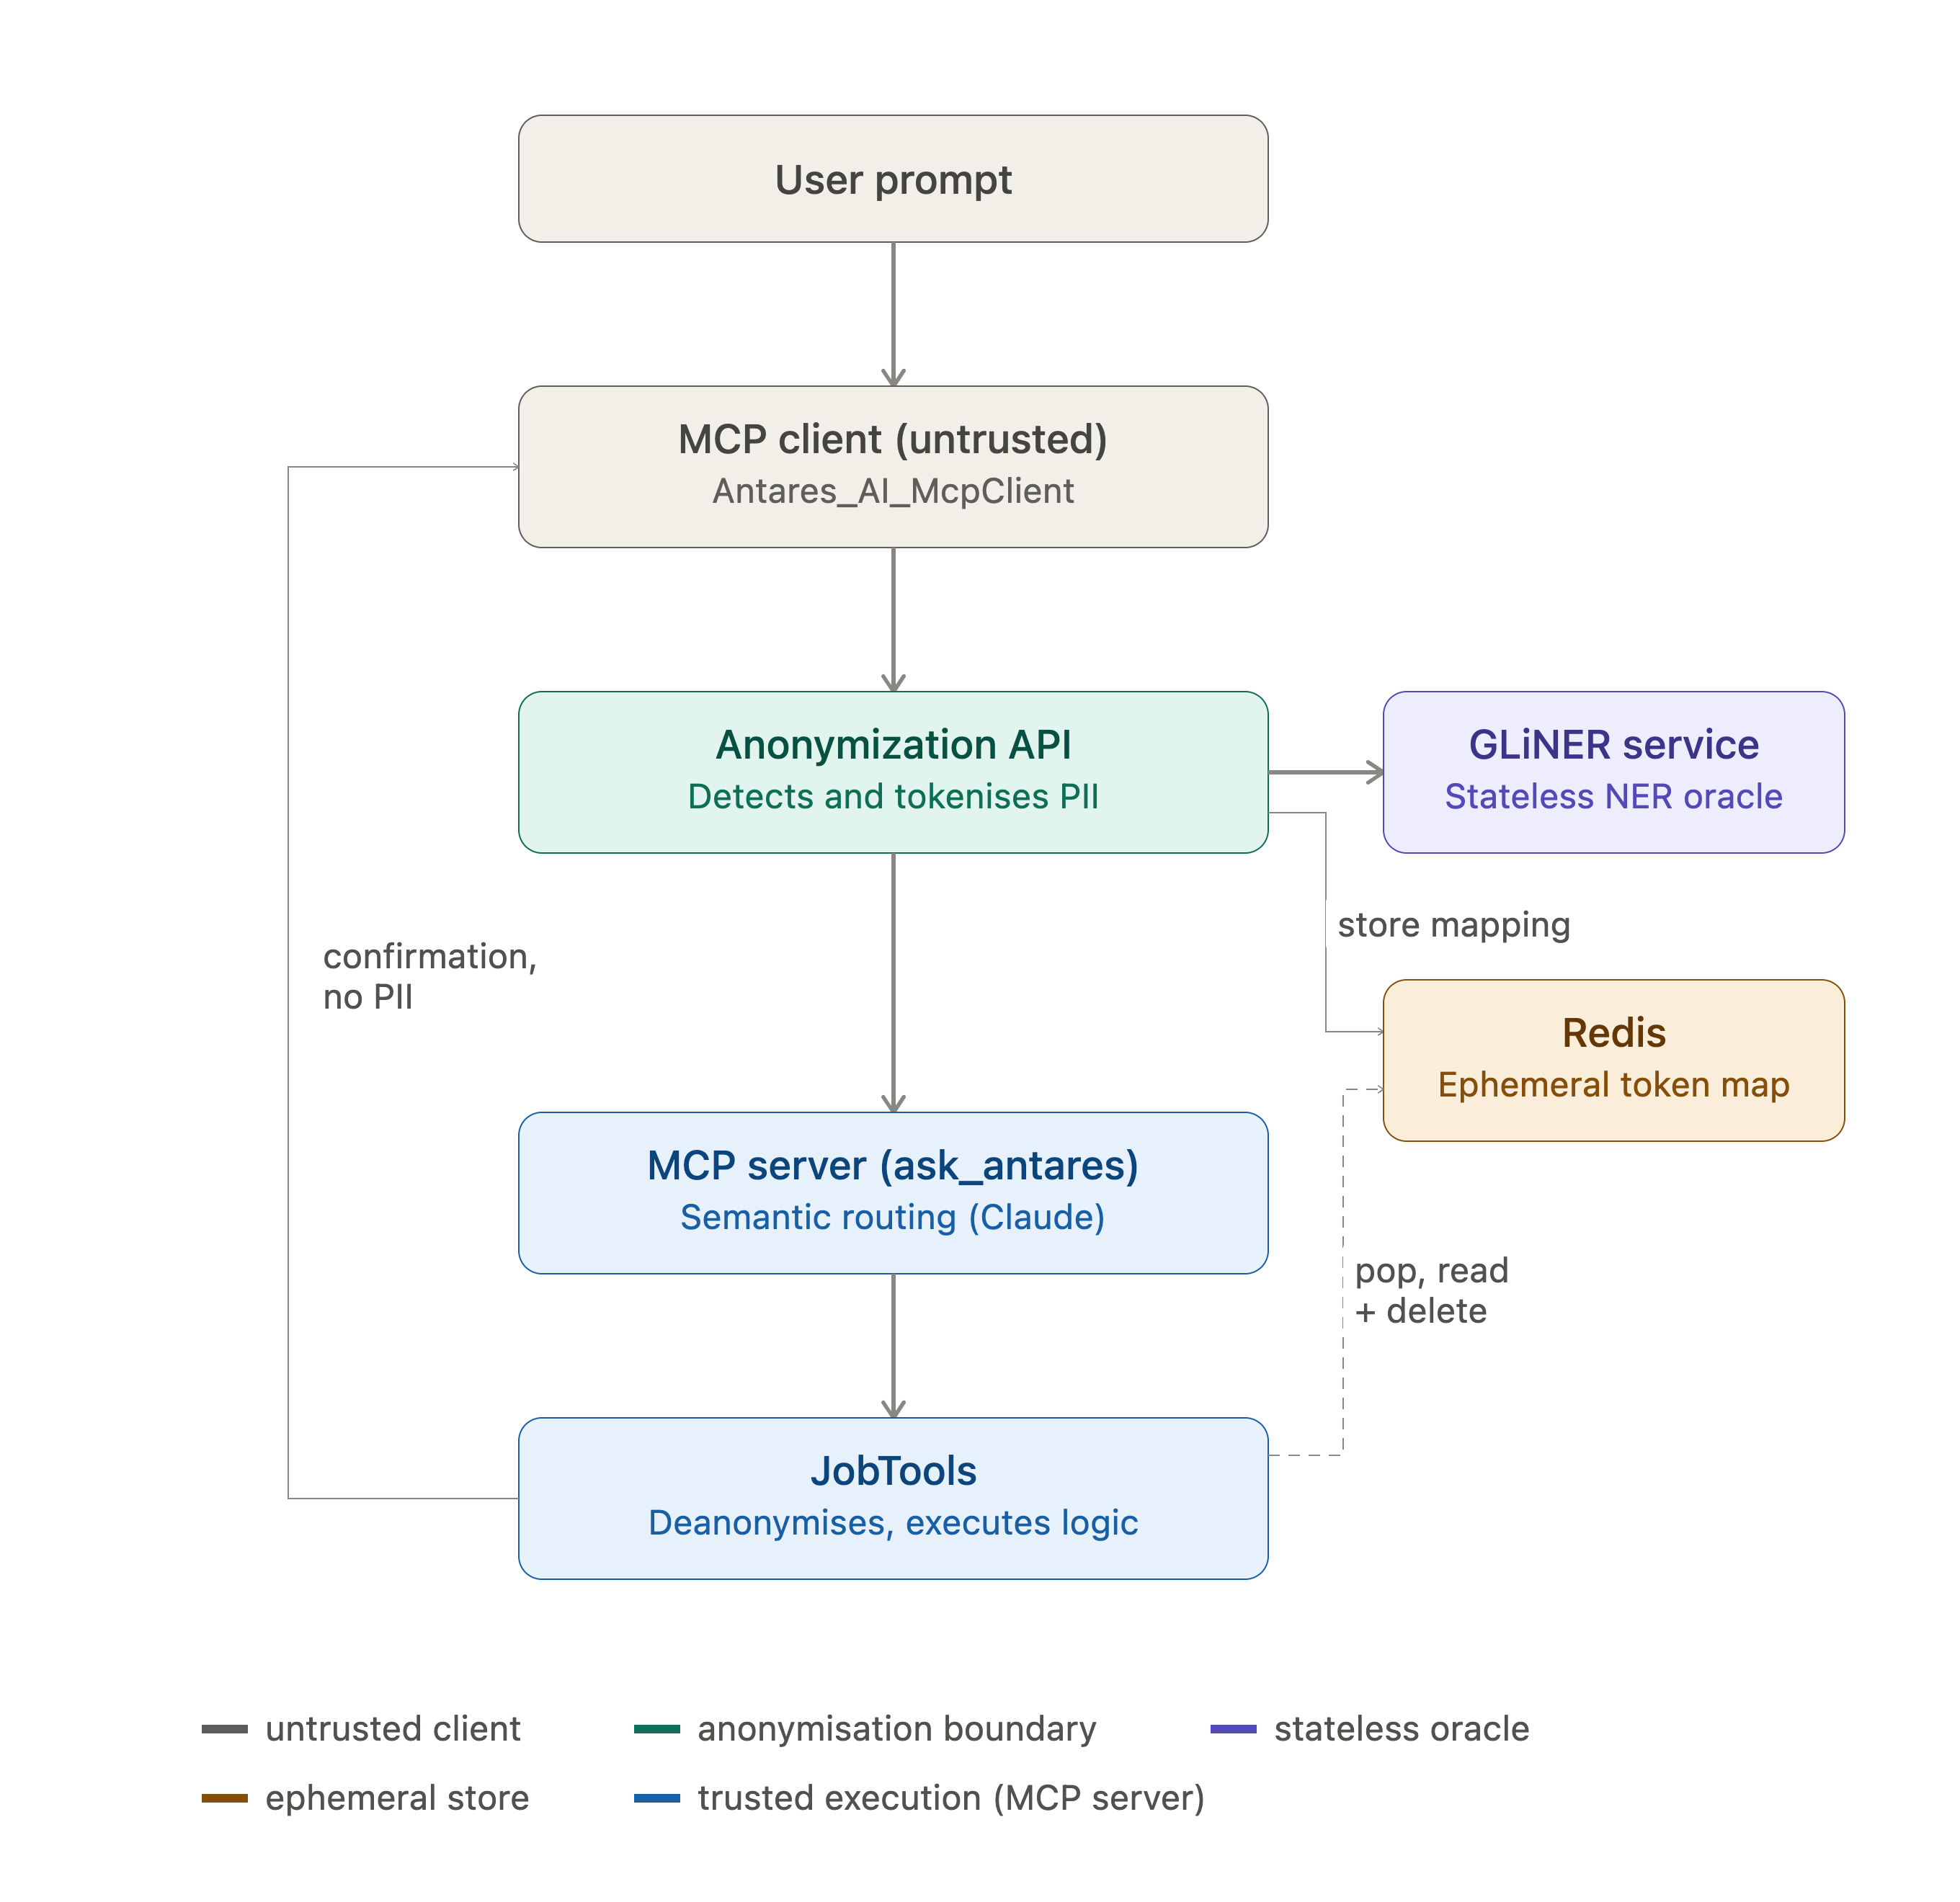
\includegraphics[width=\textwidth]{Immagini/antares_ai_secure_flow_corrected}
    \caption{Runtime architecture of Antares AI. The client anonymises the user prompt before crossing the MCP boundary. The MCP server routes the anonymised request via Claude and executes the selected business tool server-side, where PII is restored from the Redis context. The client receives only a hardcoded confirmation string.}
    \label{fig:runtime_flow}
\end{figure}

The four services and their roles are summarised in Table~\ref{tab:services}.

\begin{table}[htbp]
\centering
\caption{Antares AI runtime services}
\label{tab:services}
\begin{tabular}{llll}
\hline
\textbf{Service} & \textbf{Stack} & \textbf{Port} & \textbf{Role} \\
\hline
MCP Client & C\#/.NET~10 & --- & Request orchestration and test harness \\
Anonymization API & C\#/.NET~10 & 5292 & PII detection, tokenisation, context storage \\
GLiNER Service & Python/FastAPI & 5100 & Named entity recognition \\
MCP Server & C\#/.NET~10 & 5001 & LLM routing and business tool execution \\
\hline
\end{tabular}
\end{table}

The communication topology mirrors the system's trust model. The MCP client is an untrusted endpoint: it never receives real personnel data, and the only thing it sees is a hardcoded Italian confirmation string. The anonymisation API sits at the client-side boundary, processing the raw prompt and issuing a session token (\texttt{contextId}) that indexes the stored mapping. The GLiNER service is a stateless NER oracle; it knows nothing about tokens, Redis, or business context. The MCP server is the trusted execution boundary: it receives only anonymised prompts, routes them via Claude, restores PII server-side, and executes business tools against real data.

Redis~\cite{redis2009} runs at port~55000 as the ephemeral context store. It is not reachable from the client and is accessible only to the anonymisation API (writing) and the MCP server (reading and consuming).

The architectural invariant (no PII crosses the MCP boundary) is enforced at the interface between client and server. The \texttt{ask\_antares} tool accepts an anonymised prompt and a \texttt{contextId}; it never receives raw PII. The client calls the anonymisation API first, gets an anonymised prompt and a \texttt{contextId}, and only then constructs the tool call. PII restoration from the \texttt{contextId} happens inside the server's trusted boundary, after the routing decision has been made.

% ==========================================
\section{Component Design}
\label{sec:arch_components}

\subsection{The MCP Client Orchestrator}
\label{subsec:arch_mcp_client_orchestrator}

The MCP client (\texttt{Antares\_AI\_McpClient}) is a .NET~10~\cite{dotnet10} console application that orchestrates the end-to-end request lifecycle. In the current system it serves as both the reference client implementation and the integration test harness for the three use case scenarios.

Its responsibilities are deliberately minimal. It constructs a natural language prompt, submits it to the Anonymization API, and then calls \texttt{ask\_antares} on the MCP server with the anonymised prompt and \texttt{contextId}. The client performs no business logic and holds no sensitive data; it can't observe PII because it never calls a deanonymisation endpoint or touches the Redis context.

Communication with the MCP server uses the HTTP/SSE transport via \texttt{ModelContextProtocol.Core}. Communication with the Anonymization API uses a strongly typed HTTP client generated by NSwag~\cite{nswag2015} from the API's OpenAPI specification, keeping the client's view of the API interface in sync with the server implementation automatically.

A production client would accept dynamic user input, manage multi-turn context across \texttt{contextId} sessions, and surface token placeholders in the UI as opaque references. The current implementation uses hardcoded prompts to enable deterministic integration testing.

\subsection{The Anonymization Service API}
\label{subsec:arch_anonymization_service}

The Anonymization Service (\texttt{AnonymizationServiceAPI}) is an ASP.NET Core Minimal API application that acts as the PII gateway between client and server. It exposes three REST endpoints: \texttt{GET /anonymize}, \texttt{POST /anonymize-into-context}, and \texttt{POST /deanonymize-known}.

The primary client-facing operation is \texttt{/anonymize}. It receives a raw prompt, delegates entity detection to the GLiNER service, replaces detected entities with stable typed tokens, generates a \texttt{contextId}, stores the token-to-entity mapping in Redis, and returns the anonymised text, the \texttt{contextId}, and a detection count. The token format is \texttt{<LABEL\_NNNN>}, where \texttt{LABEL} is the uppercase entity type and \texttt{NNNN} is a zero-padded counter per label per context. This preserves entity type and cardinality while stripping identifying content.

The \texttt{/anonymize-into-context} endpoint extends an existing session by merging new token mappings into an already-issued \texttt{contextId}. This supports multi-turn interactions where a follow-up request introduces a new entity that must be pseudonymised within the same operational context.

The \texttt{/deanonymize-known} endpoint is the server-facing operation. It receives an anonymised string and a \texttt{contextId}, retrieves the mapping from Redis via a \texttt{Pop} operation (atomic read-and-delete), and restores original values through string substitution. The one-time-use design limits the exposure window for the mapping to the minimum needed for tool execution; a repeated call with the same \texttt{contextId} will find no context and fail cleanly.

Detection is fully delegated to the GLiNER service. The separation between detection (GLiNER) and masking plus context management (Anonymization API) preserves substitutability: the NER backend can be replaced without touching the tokenisation logic.

\subsection{The GLiNER-based NER Microservice}
\label{subsec:arch_gliner_ner}

The GLiNER service (\texttt{GLiNERService}) is a Python FastAPI~\cite{fastapi2018} application that exposes a single stateless endpoint, \texttt{POST /analyze}, and a health check at \texttt{GET /health}. Its job is to apply the GLiNER model to an input text and return a list of detected entity spans with labels, character offsets, and confidence scores.

The multilingual model \texttt{urchade/gliner\_multi-v2.1}~\cite{zaratiana2023gliner} is loaded once at startup and held in memory for the process lifetime. Model weights download from HuggingFace on first run and are cached locally; subsequent starts use the cached copy.

The service is a dumb NER oracle. It receives text and labels, runs the model, returns spans. All policy decisions (which labels to request, what confidence threshold to apply, how to handle overlapping spans) are made by the Anonymization API, which configures the \texttt{/analyze} call accordingly. This keeps the GLiNER service simple and reusable.

Three post-processing stages run within the Anonymization API before token substitution. Raw predictions are normalised: invalid offsets, missing labels, and out-of-bounds spans are discarded. Low-quality entities are filtered out: spans below the 0.45 confidence threshold, spans shorter than three characters, and spans matching an Italian stopword blocklist are removed. Overlapping predictions are deduplicated, keeping the higher-confidence, longer span. The result is a clean, non-overlapping list of entity spans ready for replacement.

\subsection{The Antares MCP Server}
\label{subsec:arch_antares_mcp_server}

The MCP server (\texttt{Antares\_AI\_McpServer}) is the trusted execution boundary. It exposes the \texttt{ask\_antares} routing tool, calls the Claude API for semantic routing, and executes the selected business tool against the Miorelli data layer.

Tools are registered via \texttt{ModelContextProtocol.AspNetCore}, which generates MCP-compliant schemas from C\# class and method annotations. Two types are registered: \texttt{AntaresTools} (exposing \texttt{ask\_antares}) and \texttt{JobTools} (exposing the three business operations). The \texttt{JobTools} methods are not called directly by the MCP client; Claude invokes them through function-calling within an \texttt{ask\_antares} execution.

The server calls Claude~Sonnet~4.6 via the \texttt{Anthropic.SDK} client. The system prompt defines Claude's role as a semantic router, lists the available sub-tools with descriptions, and enforces privacy constraints: the model must not infer or reveal PII from tokens, must forward the \texttt{contextId} to the selected sub-tool, and must include the sub-tool's result string verbatim in its response. A retry loop with exponential backoff handles transient \texttt{overloaded\_error} responses, retrying up to four times before returning an error message.

The data access layer is abstracted behind \texttt{IMiorelliService}. The current implementation registers \texttt{MiorelliServiceStub}, which throws \texttt{MiorelliClientNotAvailableException} on every call; each business tool catches this and falls back to static mock data from \texttt{MiorelliMockDataProvider}. Switching to the real Miorelli tenant requires changing one line in \texttt{program.cs}: registering \texttt{AntaresMiorelliClient} instead of the stub. No tool code changes. This design is discussed in Chapter~\ref{ch:implementation}.

% ==========================================
\section{Data Flow and Lifecycle of a Request}
\label{sec:arch_data_flow}

This section traces a user request from natural language prompt to confirmation response. Use Case~A (finding the nearest available workers to a named client site) serves as the concrete example.

\subsection{Tokenisation and Ephemeral Context Storage}
\label{subsec:arch_tokenization_redis}

The lifecycle begins when the MCP client constructs a natural language prompt. For Use~Case~A, a typical prompt is: \emph{``Trova i lavoratori più vicini al cantiere Bergamo Via della Fonda~5 Giulia S.r.l.\ entro~15~km. Risolvi tutti i GUID internamente.''} This contains two PII spans: a location name (\emph{Bergamo Via della Fonda~5}) and a company name (\emph{Giulia S.r.l.}).

The client calls \texttt{GET /anonymize}. The API calls the GLiNER service, receives entity predictions, runs the three-stage filtering pipeline, and sorts surviving entities by character offset in reverse order. Replacements are applied right-to-left to avoid invalidating offsets of earlier spans. The location becomes \texttt{<LOCATION\_0001>} and the company becomes \texttt{<ORGANIZATION\_0001>}.

The mapping \texttt{\{"<LOCATION\_0001>": "Bergamo Via della Fonda 5", "<ORGANIZATION\_0001>": "Giulia S.r.l."\}} is stored in Redis under \texttt{anon:context:\{contextId\}}, where \texttt{contextId} is a freshly generated UUID. The API returns the anonymised prompt and the \texttt{contextId} to the client. No PII is in the response; the client holds only an opaque session identifier.

Redis is the right tool here for practical reasons: its in-memory architecture gives sub-millisecond read and write latency, which matters in a synchronous request pipeline. Its native hash type matches the token-map structure directly, and its in-memory-with-optional-persistence model suits ephemeral session data that does not need to survive a service restart.

\subsection{Isolated Semantic Routing}
\label{subsec:arch_semantic_routing}

The client constructs the \texttt{ask\_antares} tool call with the anonymised prompt and \texttt{contextId}, dispatching it over HTTP/SSE. At this point the MCP boundary has been crossed and no PII is in transit.

The \texttt{ask\_antares} implementation builds a Claude API call. The system prompt defines Claude's role as an Italian-language semantic router, provides the JSON schemas of the available sub-tools, and specifies the expected response format. The anonymised user prompt becomes the user message.

Claude's task is intent classification (which sub-tool?) and parameter extraction (what values, in anonymised form?). For Use~Case~A it classifies the intent as \texttt{get\_nearest\_workers\_to\_cantiere} and extracts \texttt{cantiereName = "<LOCATION\_0001>"} and \texttt{context\_id = \{contextId\}}. It doesn't try to resolve the token; it works entirely with the pseudonymised representation.

The Claude API returns a structured tool call rather than free text. The \texttt{Microsoft.Extensions.AI} abstraction intercepts it, locates the registered \texttt{GetNearestWorkersToCantiere} method, and invokes it with the extracted parameters. The Redis context is not touched during this phase.

\subsection{Server-Side Deanonymisation and Tool Execution}
\label{subsec:arch_deanonymization}

The \texttt{GetNearestWorkersToCantiere} method is the first point where PII re-enters the system. Its first action is to call \texttt{DeanonymizeAsync}, which posts to \texttt{/deanonymize-known} with the token \texttt{"<LOCATION\_0001>"} and the \texttt{contextId}. The API atomically reads and deletes the context from Redis and returns the original value: \texttt{"Bergamo Via della Fonda 5"}. The Redis context no longer exists after this call.

The deanonymised value drives the business logic entirely within the server's trusted boundary. The method resolves the caller's authorised cantieri via the Miorelli service layer, locates the matching site, retrieves assigned workers via the \texttt{PULITO\_DA} relation, computes Haversine distances from each worker's registered coordinates to the site's GPS coordinates, and filters and ranks results by distance within the specified radius.

The full report, containing real names, phone numbers, distances, and status information, is written to a timestamped file in the server's local \texttt{logs/} directory. It is never transmitted to the client. The method returns a hardcoded Italian confirmation string: \emph{``Operazione completata con successo.''} Claude includes this verbatim in its final response.

The client receives a short text block with no PII. The invariant holds across the entire lifecycle: no personally identifiable information crossed the MCP boundary, and a complete, accurate operational result was produced server-side.


\input{capitoli/implementation}

\input{capitoli/validation}

\chapter{Discussion and Future Work}
\label{ch:discussion}

This chapter reflects on what the implementation and validation described in the previous chapters actually established, and where the current system falls short of what running in production would require. Section~\ref{sec:discussion_security_complexity} weighs the security properties the anonymisation pipeline provides against the architectural complexity it adds, including the prototype-scope gaps already flagged in earlier chapters rather than solved problems. Section~\ref{sec:discussion_validation_limitations} separates what typed schemas and deterministic code actually guarantee from what was measured, and names the routing model's temperature setting as an open methodological question rather than an implicit assumption. Section~\ref{sec:discussion_production_migration} discusses what remains before the mock Miorelli backend can be replaced with the production system. Section~\ref{sec:discussion_redis_scalability} considers how the Redis-based context store would need to change under concurrent, multi-tenant load. Section~\ref{sec:discussion_future_extensions} closes the chapter with two possible extensions: multimodal (voice) input and locally hosted models.

% ==========================================
\section{Security vs.\ Complexity Trade-offs}
\label{sec:discussion_security_complexity}

The anonymisation pipeline's privacy protections stop short of what a production deployment would require in two related places. The Redis context holding token-to-entity mappings (Section~\ref{subsec:impl_token_reinjection}) has no time-to-live configured. A mapping is removed only when \texttt{Pop} is actually called during a successful server-side deanonymisation; a request that errors out before that point, or a client session that is abandoned mid-flow, leaves its mapping in Redis with no expiry, bounded in practice only by the process's own lifetime. The per-request reports written to \texttt{JobTools}'s local \texttt{logs/} directory (Section~\ref{sec:impl_jobtools}) sit on the other side of the same gap: they contain real names, phone numbers, and distances, are never transmitted anywhere and were never intended to be, but they are also an unencrypted, access-uncontrolled, retention-unmanaged record on local disk.

Neither gap was addressed during the internship, and that was a deliberate scope decision rather than an oversight. The system runs as a local proof of concept: Redis has no persistence volume mounted, so every context is cleared the moment the container stops regardless of whether \texttt{Pop} ever ran, and the log files exist on a machine no one outside the development team has access to. What the internship needed to demonstrate was that reversible pseudonymisation and its MCP-based orchestration work correctly end to end, not that the system already meets the retention and access-control standards a production deployment would be held to. Closing this gap would mean configuring an explicit time-to-live on the Redis context matched to the maximum reasonable lifetime of a single request, defining a retention and deletion policy for the log files, and encrypting them at rest; none of this requires redesigning the architecture described in Chapter~\ref{ch:architecture}, only additional operational hardening on top of it.

% ==========================================
\section{Validation Methodology Limitations}
\label{sec:discussion_validation_limitations}

Two claims elsewhere in this thesis rest on single-pass evidence rather than systematic measurement, and it is worth stating that distinction plainly rather than leaving it implied. Typed tool schemas (Section~\ref{subsec:impl_csharp_reflection}) guarantee that a call Claude makes is well-formed, a valid tool name with parameters of the right type. They guarantee nothing about whether that call was the right one. Whether Claude selected the correct sub-tool for a given request, or extracted the correct parameter from an anonymised prompt, is a separate question no schema can answer, and no systematic test suite in this thesis answers it either: the worked examples in Chapter~\ref{ch:usecases} show each use case executing correctly once, not routing accuracy measured across a representative set of Italian prompts.

The same gap compounds with a second one. \texttt{AskAntares} calls Claude at temperature 1.0 (Section~\ref{subsec:impl_ask_antares}), a sampling setting under which the same prompt is not guaranteed to produce the same output on repeated calls. A single successful trace, of the kind Chapter~\ref{ch:usecases} presents, says nothing about whether that same prompt would route identically on a second or third attempt. Establishing routing accuracy as a general property of the system, rather than a property observed once per use case, would require running each test prompt multiple times and reporting both the correctness of each run and the consistency across runs, which this thesis did not do.

\iffalse
\section{Moving from Mock Providers to Production Databases}
\label{sec:discussion_production_migration}
% Write your text here discussing the steps, risks, and considerations involved in replacing the Miorelli stub interface with live production data sources

\section{Scalability of the Redis Context Mapping}
\label{sec:discussion_redis_scalability}
% Write your text here analysing the scalability characteristics of the ephemeral Redis token store under concurrent load, and potential strategies for horizontal scaling or alternative backends

\section{Future Extensions}
\label{sec:discussion_future_extensions}

\subsection{Handling Multimodal Inputs (Voice)}
\label{subsec:discussion_voice}
% Write your text here discussing how the anonymization and routing pipeline could be extended to support voice input, including speech-to-text transcription, spoken PII detection, and real-time processing constraints

\subsection{Transitioning to Local/On-Premise Models}
\label{subsec:discussion_local_models}
% Write your text here discussing the feasibility and implications of replacing the external Claude API with locally hosted or on-premise LLMs, including privacy benefits, hardware requirements, and performance trade-offs
\fi

\chapter{Conclusions}
\label{ch:conclusions}

\section{Summary of the Work}
\label{sec:conclusions_summary}

Chapter~\ref{ch:introduction} established three foundational research questions under a strict constraint: an LLM performing semantic routing on natural-language workforce requests while excluding personal data from its active context, yet maintaining the operational precision required for an administrator to act upon the output without manual verification. The subsequent chapters addressed these inquiries empirically through the implementation and validation of a functional system rather than relying exclusively on theoretical arguments.

The first question investigated the distribution of responsibilities among the client, the anonymisation layer, the LLM, and the business logic server to structurally minimise PII exposure rather than depending on operational policy. The four-tier topology introduced in Chapter~\ref{ch:architecture} satisfies this requirement. The Model Context Protocol (MCP) client anonymises requests via the Anonymisation Service prior to external transmission. Specifically, GLiNER detects sensitive entities, the Anonymisation Service substitutes them with typed and numbered tokens, and the mappings are persisted within Redis under unique context identifiers. Consequently, \texttt{ask\_antares} receives solely the tokenised representation and the context identifier. \texttt{JobTools} restores original values server-side at the point of execution after Claude generates its routing decision (Section~\ref{sec:arch_privacy_by_design}).

By design, no component upstream of \texttt{JobTools} possesses both a token and its underlying plaintext value, ensuring the model interacts exclusively with tokenised artifacts. Chapter~\ref{ch:usecases} evaluated the practical effectiveness of this architecture, revealing that detection recall governs overall privacy guarantees. Scanning fifty test prompts for literal plaintext strings exposed unmasked PII in two instances. Both cases stemmed from specific detection failures by GLiNER---wherein entities were overlooked entirely rather than leaking through already-established tokens (Section~\ref{subsec:usecases_llm_audit}).

The second question examined the detection tier, evaluating whether a zero-shot, multilingual Named Entity Recognition (NER) model could reach practically usable recall on Italian business terminology after the rule-based alternative, Presidio, proved inadequate (Section~\ref{subsec:impl_gliner_pivot}). Across 82 labelled entity spans distributed through 50 prompts, GLiNER attained 93.8\% precision and 91.5\% recall on the coverage metric, which dictates whether PII can infiltrate the LLM context (Table~\ref{tab:gliner_metrics}). The seven missed spans were not randomly distributed; four shared a common structural origin linked to Italian date-range expressions structured as ``dal X al Y'', as detailed in Table~\ref{tab:gliner_fn}.

The third question analysed the operational cost that reversible tokenisation imposes on system correctness. Twelve end-to-end test scenarios across three distinct use cases---each verified against an independent reference implementation sharing no common codebase---exhibited complete parity (Tables~\ref{tab:uca_e2e}, \ref{tab:ucb_e2e}, and \ref{tab:ucc_e2e}). Routing accuracy over tokenised inputs reached 95.2\% using the log-diffing evaluation methodology. Manual inspection of the single discrepancy confirmed that Claude selected the appropriate tool before encountering a legitimate business logic exception prior to log generation, indicating a methodological limitation rather than a routing failure (Table~\ref{tab:routing_summary}). Furthermore, running 21 distinct prompts across five repetitions each at a sampling temperature of 1.0 yielded identical routing selections in every trial. Within this test set, the privacy layer did not cost measurable correctness: routing and end-to-end results matched the reference implementation and stayed stable across repeated sampling, though the test set is 21 hand-built prompts, not a claim covering the full space of real user phrasing.

The validation phase also uncovered minor discrepancies in earlier architectural descriptions. Chapter~\ref{ch:architecture} originally stated that GLiNER split the canonical Bergamo prompt into two location tokens; however, telemetry data for Table~\ref{tab:routing_summary} confirmed that three tokens were generated due to compound site phrasing. While minor, this correction underscores a broader principle: architectural specifications that remain unchecked against running systems frequently harbor inaccuracies discoverable solely through direct runtime observation.

These results warrant careful qualification. GLiNER's coverage recall of 91.5\% dictates the practical ceiling of the system's privacy guarantees, as undetected entities reach the model unmasked (Section~\ref{subsec:usecases_llm_audit}). Furthermore, the Redis context store lacks an active time-to-live configuration, and server-side deanonymisation fails to purge read mappings, causing token associations to persist throughout the process lifecycle beyond failed or abandoned requests (Section~\ref{sec:discussion_security_complexity}). Additionally, the absence workflow for Use Case C remained unexercised due to test windows falling outside the mock dataset's absence-ticket interval (Section~\ref{sec:usecases_holiday_request}). Finally, evaluations utilised a mock Miorelli backend rather than a live production tenant, a scoping decision agreed upon with the enterprise partner to prioritise privacy-layer validation (Section~\ref{sec:intro_contributions}).

\section{Final Remarks on Enterprise AI Adoption}
\label{sec:conclusions_final_remarks}

The General Data Protection Regulation (GDPR) draws a definitive legal distinction between pseudonymisation and anonymisation. As outlined in Section~\ref{subsec:background_pii_definitions}, substituting a proper name with \texttt{<PERSON\_0001>} relocates personal data rather than destroying it---transferring information from an uncontrolled third-party provider infrastructure to an internal Redis repository managed by the organisation~\cite{gdpr2016}. This distinction dictates how the conclusions of this work generalise. Mitigating LLM exposure does not extinguish core regulatory obligations; instead, it shifts accountability to the storage layer of the token mappings, which demands identical engineering rigor, access control, and retention management as raw personal data~\cite{enisa2019pseudonymisation}. The absence of an automated time-to-live policy within the project's Redis store is exactly this risk in practice: a boundary between models and sensitive data does not, on its own, secure the data store behind that boundary.

The Model Context Protocol's separation of host, server, and model roles~\cite{anthropic2024mcp} provided an established framework for integrating this boundary without building infrastructure from scratch. The empirical contribution of this thesis lies in validating that these enforcement mechanisms hold under operational testing rather than relying solely on protocol documentation (Section~\ref{sec:usecases_validation}). Systematic reviews of the broader MCP ecosystem indicate that few production deployments enforce these available safeguards~\cite{hou2025mcpsecurity}. Antares AI successfully implements model isolation for PII while sharing common operational vulnerabilities---such as local log retention, unencrypted storage at rest, and insufficient access controls---identified across the wider MCP landscape.

Section~\ref{sec:background_sota} did not find a system in the literature it reviewed that combines local detection, reversible tokenisation, external semantic routing, and deterministic server-side execution alongside a validated correctness benchmark. Antares AI closes part of that gap, within the scope of that same review. The validation dataset reflects one specific enterprise platform rather than a cross-domain general-purpose benchmark. However, the foundational methodology remains broadly reusable: detecting PII locally, tokenising reversibly, routing via tokens externally, executing within trusted boundaries, and directly measuring detection recall. The specific numerical accuracy metrics are tied to this dataset and prompt distribution, whereas the overarching architectural pattern offers a viable blueprint for alternative domains and backends.

The replacement of Presidio with GLiNER (Section~\ref{subsec:impl_gliner_pivot}) carries implications extending beyond technical performance. The initial architecture was approved using Presidio, yet subsequent testing against real Italian enterprise inputs necessitated its replacement due to insufficient recall. Implementing privacy-by-design~\cite{cavoukian2009privacy} in practice required discarding an approved component following empirical validation. This mirrors counterfactual analyses of privacy failures at major technology firms, where abstract commitments frequently fail when weighed against specific engineering decisions~\cite{rubinstein2013counterfactual}. Similarly, Use Case C's authorisation gate depends on hardcoded identities that must be re-engineered once real identity providers are introduced (Section~\ref{sec:discussion_production_migration}). These observations suggest that enterprise privacy engineering is less constrained by initial architectural planning than by the organisational willingness to revise components when confronted with operational realities.

The findings support one precise claim: privacy and capability are compatible in language-model-powered enterprise systems under three preconditions. The boundary separating models from sensitive data must be structural rather than presumptive. Detection recall must be measured, not assumed. Downstream business logic must stay deterministic and auditable rather than delegated to a probabilistic model. Antares AI met these three conditions within one workforce management context, on the dataset and prompts this thesis tested. Whether the same conditions hold in other domains, languages, or with other model providers is untested and open for future work.

\printglossaries
\addcontentsline{toc}{chapter}{Glossary}

\printnomenclature
\addcontentsline{toc}{chapter}{Nomenclature list}
